% =====================================================================
%  2. Analyse exploratoire des données (EDA)
% =====================================================================
\clearpage
\section{Analyse exploratoire des données}
\label{sec:eda}

L'objectif de l'analyse exploratoire (notebook \notebook{01\_eda.ipynb}) est de
\emph{maîtriser} la base avant toute modélisation : savoir ce qui est mesuré,
dans quelle unité, avec quelle fiabilité, et identifier les tâches de
prétraitement nécessaires. Aucune imputation ni transformation apprise n'est
appliquée à ce stade.

\subsection{Source et structure de la base}

La base publique \emph{MAP\_DATA\_WELD} de l'université de Cambridge rassemble
des dépôts de métal fondu de soudures d'acier issus de nombreuses publications~\cite{cool_welddb,cool_1996}.
L'archive téléchargée par \fichier{scripts/download\_data.py} est vérifiée par
somme de contrôle SHA-256 ; le fichier de données \fichier{welddb.data}
(empreinte \texttt{eb46df81\ldots 676ac1}) contient \textbf{1\,652 lignes et
44 colonnes} séparées par des espaces, sans en-tête. La documentation source
définit l'ordre et les unités des colonnes, résumés au \cref{tab:structure}
(dictionnaire complet en \cref{annexe:variables}).

\begin{table}[htbp]
\centering
\small
\caption{Familles de variables de la base et unités documentées.}
\label{tab:structure}
\begin{tabularx}{\textwidth}{@{}l c L l@{}}
\toprule
Famille & Colonnes & Variables & Unité \\
\midrule
Composition principale & 12 & C, Si, Mn, S, P, Ni, Cr, Mo, V, Cu, Co, W & \% massique \\
Éléments traces        & 9  & O, Ti, N, Al, B, Nb, Sn, As, Sb & ppm massiques \\
Paramètres de soudage  & 7  & courant, tension, type de courant, polarité, apport thermique, température entre passes, procédé & A, V, --, --, kJ/mm, °C, -- \\
Traitement thermique (PWHT) & 2 & température, durée & °C, h \\
Propriétés mécaniques  & 8  & \YS, \UTS, allongement, réduction de section, température et énergie Charpy, dureté, FATT50 & MPa, MPa, \%, \%, °C, J, kg/mm$^2$, ? \\
Microstructure         & 5  & ferrite primaire, ferrite à seconde phase, ferrite aciculaire, martensite, agrégat ferrite-carbure & \% \\
Identifiant            & 1  & \texttt{weld\_id} (référence de la source) & -- \\
\bottomrule
\end{tabularx}
\end{table}

Les unités sont très hétérogènes : pourcentages massiques, ppm, ampères, volts,
kJ/mm, degrés Celsius, heures, MPa, joules. Cette hétérogénéité impose une
\textbf{standardisation} avant toute méthode sensible aux distances ou aux
échelles (ACP, $k$NN, SVR, Ridge), comme nous le verrons en \cref{subsec:standardisation}.

\subsection{Statut des mesures : absence, censure, intervalles, annotations}
\label{subsec:statuts}

La documentation précise que le symbole \texttt{N} signifie \og valeur non
rapportée \fg{} et \textbf{jamais zéro}~\cite{cool_welddb}. En lisant toutes les
colonnes comme du texte, nous avons distingué cinq statuts :
\begin{enumerate}
  \item \textbf{nombre exact} : valeur numérique sans annotation (ce qui ne veut pas dire sans incertitude expérimentale) ;
  \item \textbf{non rapporté} : symbole \texttt{N} ;
  \item \textbf{censuré} : \texttt{<L}, valeur inférieure à une limite de détection $L$ ;
  \item \textbf{intervalle} : par exemple \texttt{150-200} pour une température entre passes ;
  \item \textbf{annoté} : par exemple \texttt{67tot33res} pour l'azote (total/résiduel) ou \texttt{Hv10} pour un protocole de dureté Vickers.
\end{enumerate}

\begin{figure}[htbp]
\centering
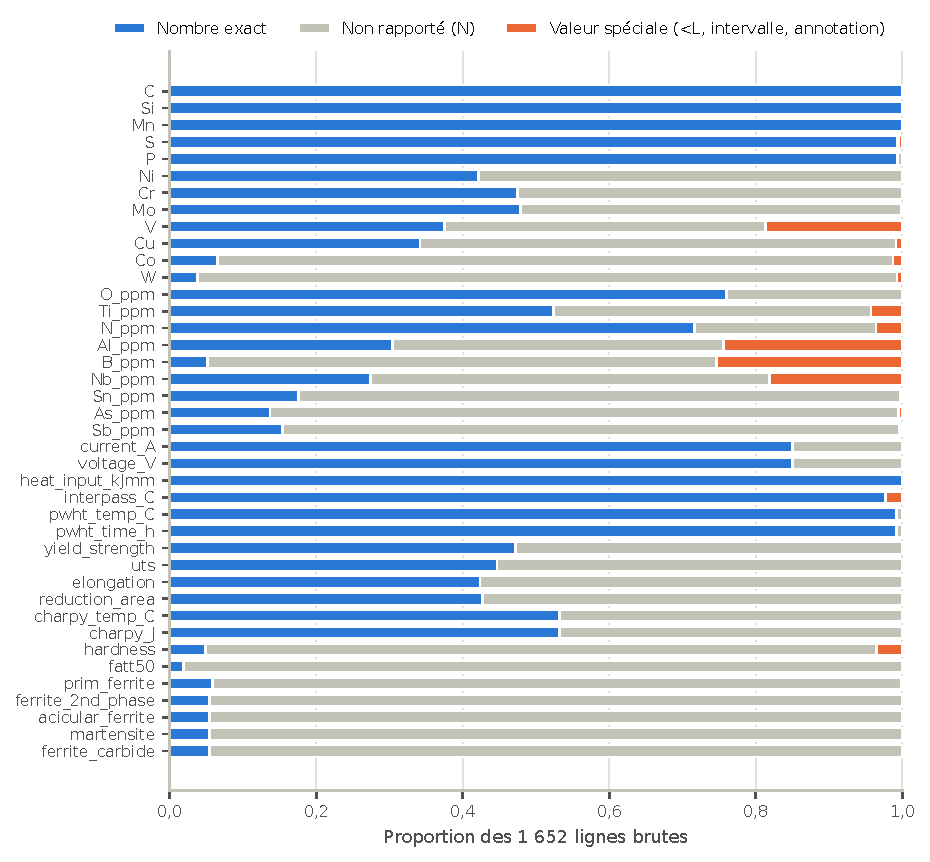
\includegraphics[width=0.93\textwidth]{eda_statuts_mesures}
\caption{Statut des 1\,652 valeurs de chaque variable numérique dans le fichier brut.
Les valeurs spéciales (censures, intervalles, annotations) sont de l'information
rapportée : elles ne doivent être confondues ni avec une absence ni avec un nombre exact.}
\label{fig:statuts}
\end{figure}

La \cref{fig:statuts} montre trois situations très différentes. Le carbone, le
silicium, le manganèse, l'apport thermique et le procédé sont renseignés sur
toutes les lignes. À l'inverse, la microstructure, la dureté et FATT50 sont
presque toujours absentes. Entre les deux, Ni, Cr, Mo, O, N, le courant et la
tension sont partiellement renseignés. \textbf{Aucune ligne n'est complète sur
les 44 colonnes} : supprimer les lignes incomplètes supprimerait toute la base.
Le \cref{tab:speciales} détaille les variables les plus concernées par la
censure ou les annotations.

\begin{table}[htbp]
\centering
\small
\caption{Variables les plus concernées par les valeurs spéciales (fichier brut, 1\,652 lignes).}
\label{tab:speciales}
\begin{tabular}{@{}lrrrr@{}}
\toprule
Variable & Nombres exacts & Censurées & Intervalles/annotations & Non rapportées \\
\midrule
Aluminium                 & 502   & 403 & 0  & 747   \\
Vanadium                  & 620   & 308 & 0  & 724   \\
Bore                      & 85    & 419 & 0  & 1\,148 \\
Niobium                   & 453   & 299 & 0  & 900   \\
Azote                     & 1\,183 & 0  & 59 & 410   \\
Température entre passes  & 1\,614 & 0  & 38 & 0     \\
Dureté                    & 80    & 0   & 58 & 1\,514 \\
FATT50                    & 31    & 0   & 0  & 1\,621 \\
\bottomrule
\end{tabular}
\end{table}

Pour l'aluminium, 44,5\,\% des valeurs rapportées sont censurées ; pour le bore,
83,1\,\%. Un histogramme calculé sur les seuls nombres exacts décrirait donc un
sous-ensemble sélectionné. Les annotations de dureté (\texttt{Hv5}, \texttt{Hv10},
\texttt{Hv30}) renvoient à des protocoles Vickers différents : les nombres
annotés vont de 143 à 467, alors que les valeurs non annotées s'arrêtent à 265.

\subsection{Identifiants, répétitions et séries}
\label{subsec:eda_series}

Les 1\,652 lignes portent \textbf{1\,490 identifiants distincts} ; 91 identifiants
apparaissent plusieurs fois et concernent 253 lignes (par exemple un même dépôt
testé en Charpy à plusieurs températures). Aucune ligne n'est un doublon exact sur
les 44 colonnes, mais \textbf{quatre lignes répètent exactement une autre ligne
lorsqu'on ignore l'identifiant} (indices bruts 393, 423, 425 et 1\,434, qui
dupliquent 333, 363, 365 et 1\,418).

Surtout, les identifiants révèlent des \textbf{séries expérimentales} : par exemple
\ident{Evans-Ni/CMn-1990/1991-0Aaw} et \ident{Evans-Ni/CMn-1990/1991-0Aawch}
appartiennent à la même étude, qui fait varier un seul élément d'alliage à
procédé et protocole constants. Les observations d'une même série partagent la
composition de base, le matériel, les opérateurs et le laboratoire d'essai.

\begin{precaution}
Si l'on mélange aléatoirement les lignes, une soudure de la validation a presque
toujours une \og sœur \fg{} de la même série dans l'entraînement. Le score obtenu
mesure alors la capacité à \emph{interpoler à l'intérieur de séries connues}, et
non à prédire une nouvelle étude. Cette observation motive la validation par
groupes décrite en \cref{sec:protocole}.
\end{precaution}

\subsection{Distributions et ordres de grandeur}

La \cref{fig:distributions} présente les distributions de neuf variables après
retrait des quatre doublons, sur les seuls nombres exacts ; le \cref{tab:ordres}
donne les ordres de grandeur correspondants.

\begin{figure}[htbp]
\centering
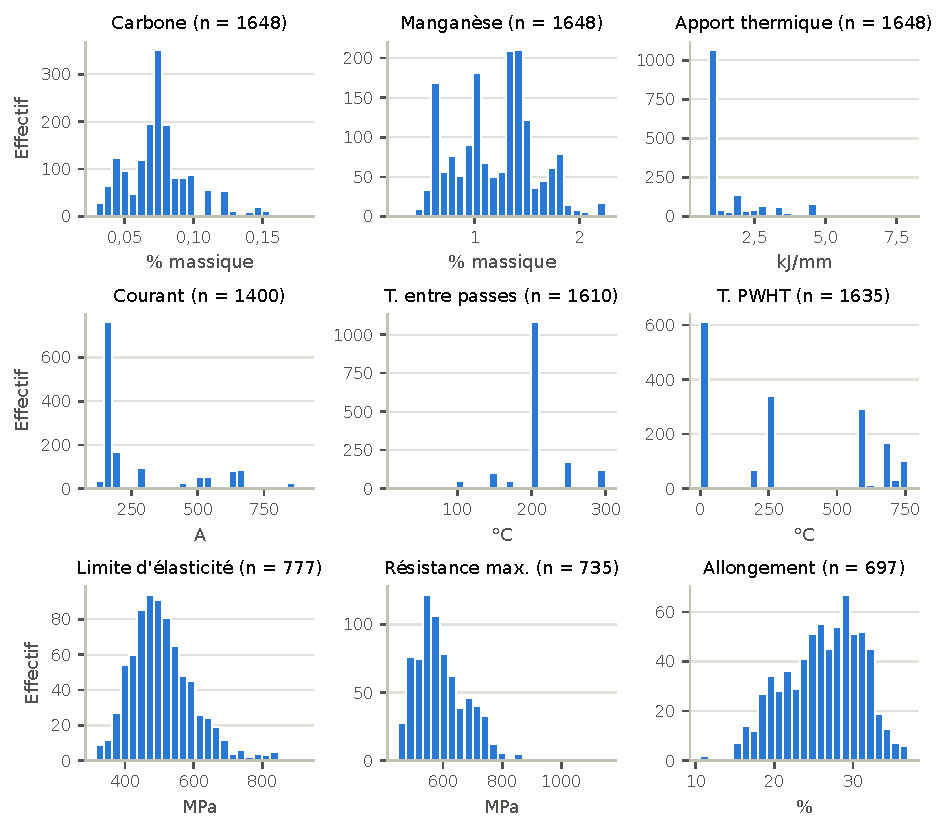
\includegraphics[width=\textwidth]{eda_distributions}
\caption{Distributions de compositions, de paramètres de soudage et de propriétés
mécaniques (nombres exacts, 1\,648 lignes dédupliquées ; $n$ = effectif disponible).
Aucune valeur extrême n'est supprimée et aucune unité n'est convertie.}
\label{fig:distributions}
\end{figure}

\begin{table}[htbp]
\centering
\small
\caption{Ordres de grandeur des principales entrées (nombres exacts, lignes dédupliquées).}
\label{tab:ordres}
\begin{tabular}{@{}llrrrr@{}}
\toprule
Variable & Unité & Effectif & Minimum & Médiane & Maximum \\
\midrule
Carbone                    & \% mass. & 1\,648 & 0,029 & 0,074 & 0,18 \\
Silicium                   & \% mass. & 1\,648 & 0,04  & 0,32  & 1,14 \\
Manganèse                  & \% mass. & 1\,648 & 0,27  & 1,27  & 2,25 \\
Nickel                     & \% mass. & 696   & 0     & 0,0675 & 3,5 \\
Chrome                     & \% mass. & 783   & 0     & 0,53  & 10,2 \\
Molybdène                  & \% mass. & 790   & 0     & 0,34  & 1,5 \\
Oxygène                    & ppm      & 1\,253 & 132  & 423   & 1\,650 \\
Azote (non annoté)         & ppm      & 1\,180 & 21   & 83    & 552 \\
Courant                    & A        & 1\,400 & 115  & 170   & 900 \\
Tension                    & V        & 1\,400 & 11,5 & 21    & 75,36 \\
Apport thermique           & kJ/mm    & 1\,648 & 0,6  & 1     & 7,9 \\
Température entre passes   & °C       & 1\,610 & 20   & 200   & 300 \\
Température PWHT           & °C       & 1\,635 & 0    & 250   & 760 \\
Durée PWHT                 & h        & 1\,635 & 0    & 2     & 24 \\
Température d'essai Charpy & °C       & 877   & $-114$ & $-40$ & 188 \\
\bottomrule
\end{tabular}
\end{table}

Plusieurs observations orientent le prétraitement :
\begin{itemize}
  \item \textbf{Distributions multimodales.} Le manganèse présente plusieurs pics ; le chrome forme des groupes autour de faibles teneurs, de 2\,\% et de 9\,\%. Ces structures traduisent un \emph{mélange de familles d'aciers et de séries expérimentales} plutôt qu'une loi unique.
  \item \textbf{Régimes de procédé.} Les 30 lignes entre 850 et 900\,A appartiennent toutes au procédé sous flux \texttt{SA}, alors que le courant médian est de 170\,A. Ces valeurs sont cohérentes avec le procédé et ne sont pas des anomalies.
  \item \textbf{Réglages répétés.} Les pics d'apport thermique (1\,kJ/mm), de température entre passes (200\,°C) et de PWHT correspondent à des réglages standard répétés.
  \item \textbf{Zéros PWHT.} 610 lignes ont le couple (0\,°C, 0\,h), qui code vraisemblablement un état brut de soudage. Ces zéros mesurés sont conservés tels quels.
  \item \textbf{Valeurs élevées regroupées.} Les plus fortes teneurs en soufre (0,14\,\%) et phosphore (0,25\,\%) apparaissent ensemble dans dix lignes d'une même série (\texttt{Mart-G\ldots}) : cela justifie un examen de provenance, pas une suppression automatique.
  \item \textbf{Cibles.} La limite d'élasticité et la résistance maximale sont unimodales avec une queue vers les fortes valeurs ; l'allongement est concentré entre 25 et 30\,\%.
\end{itemize}

\begin{decision}
Les valeurs extrêmes sont \textbf{conservées} : leur amplitude seule ne démontre
pas une erreur, et elles appartiennent souvent à un procédé ou à une série
identifiable. Supprimer ces points réduirait artificiellement la diversité des
conditions que le modèle doit apprendre.
\end{decision}

\subsection{Les absences dépendent du procédé}
\label{subsec:absences_procede}

Les absences ne sont pas réparties au hasard. La \cref{fig:absences_procede}
croise le taux de valeurs non rapportées avec le procédé de soudage (après
regroupement des seuls synonymes documentés \texttt{ShMA}$\to$\texttt{MMA} et
\texttt{SMA}$\to$\texttt{SA}).

\begin{figure}[htbp]
\centering
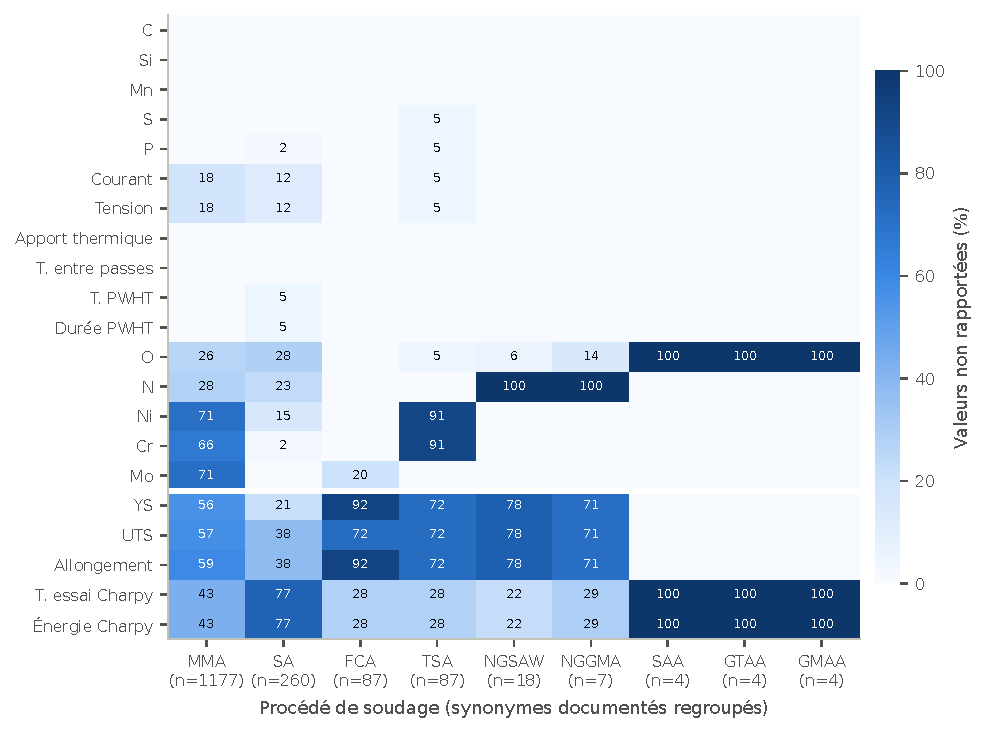
\includegraphics[width=0.95\textwidth]{eda_absences_procede}
\caption{Part de valeurs non rapportées (\%) par procédé, pour les 16 entrées
numériques retenues (haut) et les mesures cibles (bas), sur les 1\,648 lignes
dédupliquées. Cases vides : moins de 0,5\,\% d'absences.}
\label{fig:absences_procede}
\end{figure}

On y lit par exemple que l'oxygène n'est jamais rapporté pour les procédés
\texttt{SAA}, \texttt{GTAA} et \texttt{GMAA}, que l'azote manque toujours pour
\texttt{NGSAW} et \texttt{NGGMA}, que Ni et Cr manquent dans 91\,\% des lignes
\texttt{TSA}, ou que l'énergie Charpy manque dans 77\,\% des lignes \texttt{SA}.
En statistique des données manquantes, ces absences ne sont donc pas
\og complètement aléatoires \fg{} (MCAR)~\cite{little_rubin_2019} : elles dépendent
au moins du procédé et de la source.

\begin{precaution}
Une valeur imputée n'est pas une mesure. Quand l'absence dépend de la source,
l'imputation peut confondre une composition réelle avec la composition
\og typique \fg{} des autres séries. C'est pourquoi l'imputation sera ajustée dans
chaque pli d'entraînement, comparée entre plusieurs méthodes, et ses limites
explicitement testées (\cref{subsec:sensibilites}).
\end{precaution}

\subsection{Cohérence physique et unités douteuses}
\label{subsec:unites}

Les bornes physiques élémentaires sont respectées : concentrations positives,
fractions entre 0 et 100\,\%, températures au-dessus du zéro absolu. Sur les
714 lignes où les deux résistances sont présentes, \textbf{aucune limite
d'élasticité ne dépasse la résistance maximale}. Ce contrôle ne démontre
cependant pas l'homogénéité des unités. Plusieurs indices demandent un retour aux
sources :
\begin{itemize}
  \item \textbf{Aluminium} : dix lignes de la famille \texttt{EPRI-TR-101394s} contiennent 0,004 à 0,014 dans une colonne annoncée en ppm ; en \% massique, cela correspondrait à 40--140\,ppm.
  \item \textbf{Étain, arsenic, antimoine} : les mêmes 90 lignes ont simultanément des valeurs positives inférieures à 1\,ppm, motif typique d'une saisie en \% massique.
  \item \textbf{Titane et vanadium} : une valeur de 0,5\,ppm de titane, des limites \texttt{<0.01} pour Ti/Al (famille \texttt{PantK-1990}) et \texttt{<5} pour V dans une colonne en \% massique.
\end{itemize}
Rappelons que 1\,\% massique $=$ 10\,000\,ppm : multiplier toutes les petites
valeurs par 10\,000 serait une hypothèse non vérifiée. Une normalisation
statistique ne corrigerait pas non plus une erreur d'unité. Ces cellules sont donc
mises en quarantaine (\cref{subsec:nettoyage}). L'audit des publications
(\cref{subsec:charpy_audit}) a d'ailleurs confirmé qu'au moins une source
(Svensson--Gretoft) exprime Ti/Al/Sn/As/Sb en \% massique.

\subsection{Propriétés mesurées et relations entre cibles}
\label{subsec:eda_cibles}

Le \cref{tab:proprietes} recense les propriétés mécaniques candidates. Toutes
sont partiellement renseignées : chaque cible n'est disponible que pour 42 à
53\,\% des lignes.

\begin{table}[htbp]
\centering
\small
\caption{Propriétés mécaniques candidates (nombres exacts du fichier brut).}
\label{tab:proprietes}
\begin{tabular}{@{}lrrrr@{}}
\toprule
Propriété & Mesures & Minimum & Médiane & Maximum \\
\midrule
Limite d'élasticité (MPa)          & 780 & 315  & 495   & 920   \\
Résistance maximale (MPa)          & 738 & 447  & 575,5 & 1\,151 \\
Allongement (\%)                   & 700 & 10,6 & 26,8  & 37    \\
Réduction de section (\%)          & 705 & 17   & 75    & 83    \\
Énergie Charpy (J)                 & 879 & 3    & 100   & 270   \\
Dureté non annotée (kg/mm$^2$)        & 80  & --   & --    & 265   \\
FATT50 (unité non précisée)        & 31  & --   & --    & --    \\
\bottomrule
\end{tabular}
\end{table}

\begin{figure}[htbp]
\centering
\begin{minipage}[c]{0.52\textwidth}
\centering
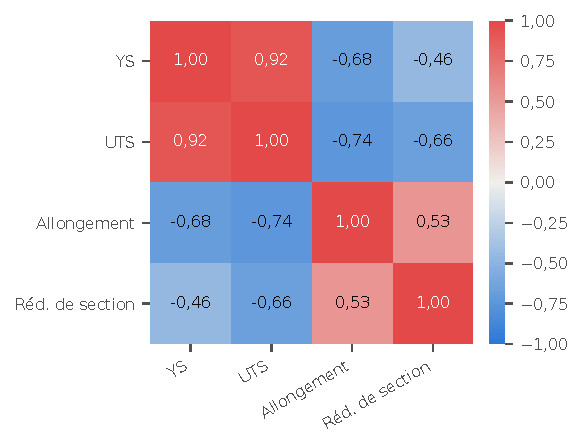
\includegraphics[width=\textwidth]{eda_correlations_cibles}
\end{minipage}\hfill
\begin{minipage}[c]{0.45\textwidth}
\caption{Corrélations de Pearson entre propriétés de traction, calculées sur les
paires observées (lignes dédupliquées). Bleu : corrélation négative ; rouge :
positive. Cette matrice décrit des dépendances par paires ; ce n'est pas une ACP.}
\label{fig:correlations}
\end{minipage}
\end{figure}

La \cref{fig:correlations} montre que \YS{} et \UTS{} sont très corrélées
($r = 0{,}915$), tandis que l'allongement leur est opposé ($r = -0{,}680$ avec
\YS, $-0{,}738$ avec \UTS) : un métal plus résistant est en moyenne moins ductile.
Ces corrélations n'autorisent pas à remplacer une cible par une autre : 0,915
laisse une part substantielle de variation propre à chacune, et résistance et
ductilité sont des informations complémentaires.

L'énergie Charpy doit toujours être lue avec sa température d'essai
(\cref{fig:charpy}). Sur 877 couples exacts dédupliqués, \textbf{355 énergies
valent exactement 100\,J et 118 valent 28\,J}. Ces valeurs correspondent à des
critères classiques de transition ductile-fragile : certaines publications
rapportent la \emph{température} à laquelle l'énergie atteint 100\,J ou 28\,J,
plutôt qu'une énergie mesurée à une température choisie~\cite{evans_1989_cr}.
Les deux protocoles produisent des points d'apparence identique dans la base.

\begin{figure}[htbp]
\centering
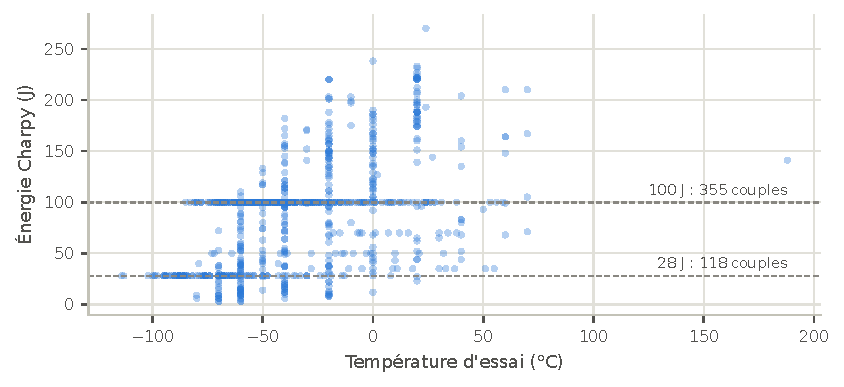
\includegraphics[width=\textwidth]{eda_charpy_couples}
\caption{Couples (température d'essai, énergie Charpy) exacts. Les lignes
horizontales à 28\,J et 100\,J concentrent 54\,\% des points, signature probable
de températures de transition plutôt que de mesures à température imposée.}
\label{fig:charpy}
\end{figure}

\subsection{Analyse en composantes principales descriptive}
\label{subsec:acp}

L'énoncé demande d'appliquer une ACP pour développer une intuition sur le
problème. L'ACP cherche les directions orthogonales de l'espace des entrées qui
expliquent le plus de variance~\cite{jolliffe_2016}. Comme les unités sont
différentes, chaque variable est d'abord \textbf{standardisée} (moyenne nulle,
écart-type unité) ; sinon le courant (centaines d'ampères) écraserait le carbone
(centièmes de pourcent).

\begin{decision}
L'ACP porte sur les \textbf{1\,339 lignes dédupliquées dont les onze entrées de
base sont des nombres exacts complets} (C, Si, Mn, S, P, courant, tension, apport
thermique, température entre passes, température et durée PWHT), \textbf{sans
imputation}. Ainsi, la structure observée n'est pas fabriquée par des valeurs
reconstruites. En contrepartie, cette sous-population peut différer de la base
entière, et l'ACP reste descriptive : elle n'est réutilisée ni pour entraîner ni
pour évaluer les modèles.
\end{decision}

\begin{figure}[htbp]
\centering
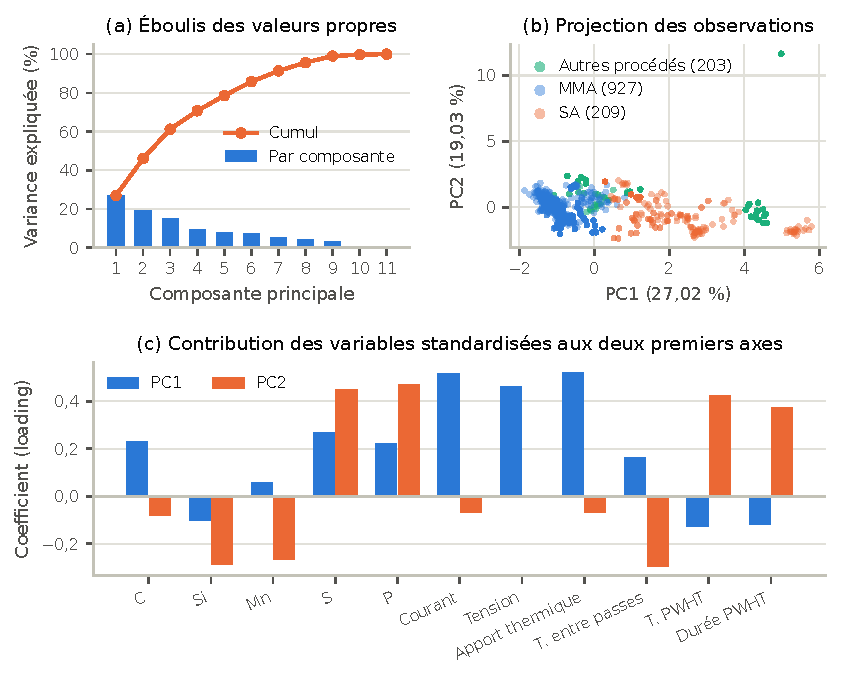
\includegraphics[width=\textwidth]{eda_acp}
\caption{ACP standardisée des onze entrées complètes (1\,339 lignes). (a) Variance
expliquée par composante et cumul. (b) Projection sur les deux premiers axes,
colorée par procédé. (c) Coefficients des variables sur les deux premiers axes.}
\label{fig:acp}
\end{figure}

Les deux premiers axes expliquent \textbf{27,02\,\%} et \textbf{19,03\,\%} de la
variance, soit 46,05\,\% cumulés ; trois axes en expliquent 61,26\,\% et il faut
huit axes pour dépasser 95\,\% (\cref{fig:acp}a). L'information est donc
\emph{répartie} sur de nombreuses directions. L'interprétation des axes
(\cref{fig:acp}c) est néanmoins éclairante :
\begin{itemize}
  \item \textbf{PC1 --- \og énergie du procédé \fg{}.} Les coefficients les plus forts sont l'apport thermique (0,52), le courant (0,52) et la tension (0,46). Cet axe sépare nettement le soudage manuel \texttt{MMA}, à faible courant, du soudage sous flux \texttt{SA}, à fort courant (\cref{fig:acp}b).
  \item \textbf{PC2 --- \og impuretés et traitement thermique \fg{}.} Le phosphore (0,47), le soufre (0,45), la température (0,43) et la durée (0,37) du PWHT s'opposent au silicium ($-0{,}29$), à la température entre passes ($-0{,}29$) et au manganèse ($-0{,}27$).
\end{itemize}
La projection montre des amas compacts correspondant à des séries et des procédés,
plutôt qu'un nuage continu. L'ACP confirme ainsi, du point de vue des entrées,
la structure en séries identifiée par les identifiants.

\begin{decision}
Aucune ACP n'est incluse dans les pipelines prédictives : les deux premiers axes
ne résument que 46\,\% de la variance, les forêts aléatoires n'en ont pas besoin,
et une réduction de dimension aurait dû être réapprise dans chaque pli. Une ACP
ajustée sur toute la base puis réutilisée en validation constituerait une fuite
d'information.
\end{decision}

\subsection{Bilan de l'analyse exploratoire}

\begin{aretenir}
\begin{itemize}[leftmargin=1.2em]
  \item La base est une \textbf{compilation de séries expérimentales} : observations apparentées, compositions multimodales, procédés déséquilibrés (\texttt{MMA} majoritaire).
  \item \texttt{N} signifie \textbf{non rapporté} ; censures, intervalles et annotations sont des informations à conserver, pas à confondre avec des nombres exacts.
  \item Les absences \textbf{dépendent du procédé et de la source} ; aucune ligne n'est complète.
  \item Quelques cellules ont une \textbf{unité douteuse} ; elles doivent être isolées sans conversion conjecturale.
  \item Les cibles sont partiellement renseignées et corrélées sans être interchangeables ; l'énergie Charpy mélange probablement plusieurs protocoles.
  \item L'ACP met en évidence un axe \og énergie du procédé \fg{} et un axe \og impuretés/PWHT \fg{}, et confirme une structure en amas liée aux séries.
\end{itemize}
\end{aretenir}
